\documentclass[10pt,a4paper]{article}
\usepackage[margin=14mm]{geometry}
\usepackage{tikz,graphicx}
\usetikzlibrary{arrows.meta}
\setlength{\parindent}{0pt}
\setlength{\parskip}{0pt}
\pagestyle{plain}
\begin{document}
{\Large\bfseries Extremal Family 1 seed graphs}\par\vspace{2mm}
{\small $m=7$; $\max_G H(G)=34$. Complete collection: 8 rooted classes and 4 underlying shapes.}\par
\vspace{1.5mm}{\small Root $0$: double circle. Port $0$: solid; port $1$: dashed. Members of each underlying shape share one vertex embedding.}\par\vspace{3mm}
\noindent\hfill
\begin{minipage}[t]{.47\textwidth}\centering
\resizebox{8.2cm}{!}{% Family 1 rooted seed, m=7; key=0001020302030405000604060105.
% Requires \usepackage{tikz} and \usetikzlibrary{arrows.meta}.
% Score and global-maximality metadata belong in the surrounding caption.
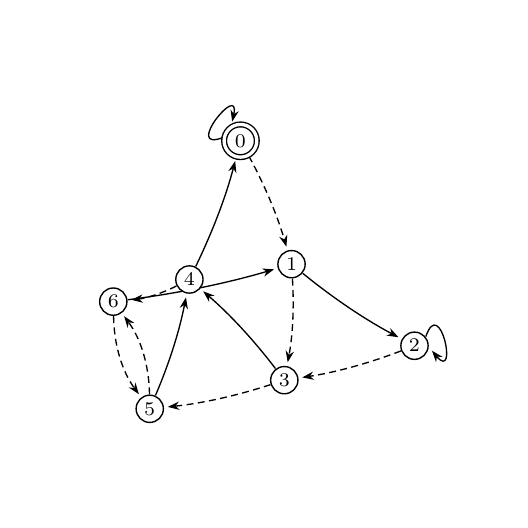
\begin{tikzpicture}[x=1cm,y=1cm,
  f1atlas state/.style={circle,draw=black,fill=white,line width=.5pt,inner sep=0pt,font=\fontsize{7}{8}\selectfont},
  f1atlas root/.style={f1atlas state,double,double distance=.42mm},
  f1atlas port0/.style={-{Stealth[length=1.45mm,width=1.05mm]},draw=black,line width=.48pt},
  f1atlas port1/.style={f1atlas port0,dash pattern=on 2.5pt off 1.6pt},
  f1atlas label/.style={font=\fontsize{6}{7}\selectfont,fill=white,inner sep=.4pt}
]
\path[use as bounding box] (-3,-3) rectangle (3,3);
% edge 0 0 0
\draw[f1atlas port0] (-0.51231,1.60760) .. controls (-1.04120,1.39929) and (-0.28849,2.32495) .. (-0.40288,1.80705);
% edge 0 1 1
\draw[f1atlas port1] (-0.19230,1.37116) .. controls (0.01056,1.00058) and (0.17009,0.61621) .. (0.28630,0.21804);
% edge 1 0 2
\draw[f1atlas port0] (0.49406,-0.12012) .. controls (0.88520,-0.43894) and (1.29010,-0.70933) .. (1.70875,-0.93128);
% edge 1 1 3
\draw[f1atlas port1] (0.36244,-0.18774) .. controls (0.38562,-0.55973) and (0.36549,-0.91373) .. (0.30203,-1.24974);
% edge 2 0 2
\draw[f1atlas port0] (2.05593,-0.92297) .. controls (2.24093,-0.39081) and (2.46965,-1.50644) .. (2.13456,-1.10266);
% edge 2 1 3
\draw[f1atlas port1] (1.74024,-1.10545) .. controls (1.31976,-1.26660) and (0.90213,-1.37872) .. (0.48736,-1.44180);
% edge 3 0 4
\draw[f1atlas port0] (0.14730,-1.32967) .. controls (-0.13508,-0.95919) and (-0.44121,-0.63213) .. (-0.77109,-0.34850);
% edge 3 1 5
\draw[f1atlas port1] (0.08369,-1.53372) .. controls (-0.35605,-1.67706) and (-0.79061,-1.77125) .. (-1.21999,-1.81630);
% edge 4 0 0
\draw[f1atlas port0] (-0.86564,-0.03187) .. controls (-0.64534,0.42325) and (-0.47828,0.86942) .. (-0.36444,1.30664);
% edge 4 1 6
\draw[f1atlas port1] (-1.11113,-0.28074) .. controls (-1.30609,-0.37841) and (-1.49673,-0.43675) .. (-1.68305,-0.45575);
% edge 5 0 4
\draw[f1atlas port0] (-1.37684,-1.67067) .. controls (-1.19863,-1.25440) and (-1.06960,-0.83906) .. (-0.98974,-0.42465);
% edge 5 1 6
\draw[f1atlas port1] (-1.45270,-1.65580) .. controls (-1.45929,-1.27556) and (-1.56676,-0.94512) .. (-1.77509,-0.66447);
% edge 6 0 1
\draw[f1atlas port0] (-1.72952,-0.45570) .. controls (-1.08441,-0.37301) and (-0.46470,-0.24403) .. (0.12961,-0.06876);
% edge 6 1 5
\draw[f1atlas port1] (-1.90943,-0.66376) .. controls (-1.90283,-1.04399) and (-1.79537,-1.37443) .. (-1.58704,-1.65509);
% state 0
\node[f1atlas root,minimum size=4.1538mm] (q0) at (-0.29757,1.56346) {$ 0 $};
% state 1
\node[f1atlas state,minimum size=3.4615mm] (q1) at (0.35096,-0.00348) {$ 1 $};
% state 2
\node[f1atlas state,minimum size=3.4615mm] (q2) at (1.91263,-1.03938) {$ 2 $};
% state 3
\node[f1atlas state,minimum size=3.4615mm] (q3) at (0.25921,-1.47650) {$ 3 $};
% state 4
\node[f1atlas state,minimum size=3.4615mm] (q4) at (-0.94607,-0.19805) {$ 4 $};
% state 5
\node[f1atlas state,minimum size=3.4615mm] (q5) at (-1.44949,-1.84038) {$ 5 $};
% state 6
\node[f1atlas state,minimum size=3.4615mm] (q6) at (-1.91263,-0.47917) {$ 6 $};
\end{tikzpicture}
}\par\smallskip
{\small (a) Rooted class 1; underlying shape 2.}\par
\end{minipage}\hfill
\begin{minipage}[t]{.47\textwidth}\centering
\resizebox{8.2cm}{!}{% Family 1 rooted seed, m=7; key=0001020304050406050600010203.
% Requires \usepackage{tikz} and \usetikzlibrary{arrows.meta}.
% Score and global-maximality metadata belong in the surrounding caption.
\begin{tikzpicture}[x=1cm,y=1cm,
  f1atlas state/.style={circle,draw=black,fill=white,line width=.5pt,inner sep=0pt,font=\fontsize{7}{8}\selectfont},
  f1atlas root/.style={f1atlas state,double,double distance=.42mm},
  f1atlas port0/.style={-{Stealth[length=1.45mm,width=1.05mm]},draw=black,line width=.48pt},
  f1atlas port1/.style={f1atlas port0,dash pattern=on 2.5pt off 1.6pt},
  f1atlas label/.style={font=\fontsize{6}{7}\selectfont,fill=white,inner sep=.4pt}
]
\path[use as bounding box] (-3,-3) rectangle (3,3);
% edge 0 0 0
\draw[f1atlas port0] (-0.32653,1.63146) .. controls (-0.87549,1.48394) and (-0.02348,2.31910) .. (-0.19538,1.81735);
% edge 0 1 1
\draw[f1atlas port1] (-0.02764,1.36377) .. controls (0.09579,1.09134) and (0.17901,0.81101) .. (0.22201,0.52280);
% edge 1 0 2
\draw[f1atlas port0] (0.10042,0.19525) .. controls (-0.19812,0.00476) and (-0.45692,-0.20942) .. (-0.67597,-0.44730);
% edge 1 1 3
\draw[f1atlas port1] (0.34862,0.13482) .. controls (0.53565,-0.18793) and (0.67588,-0.51394) .. (0.76930,-0.84321);
% edge 2 0 4
\draw[f1atlas port0] (-0.68546,-0.72896) .. controls (-0.58104,-0.80855) and (-0.47922,-0.85649) .. (-0.38002,-0.87276);
% edge 2 1 5
\draw[f1atlas port1] (-0.83363,-0.43244) .. controls (-0.83538,-0.18958) and (-0.80182,0.03214) .. (-0.73295,0.23274);
% edge 3 0 4
\draw[f1atlas port0] (0.65821,-1.00375) .. controls (0.45565,-0.93224) and (0.26238,-0.89895) .. (0.07840,-0.90390);
% edge 3 1 6
\draw[f1atlas port1] (0.65667,-1.12214) .. controls (0.34980,-1.22160) and (0.11979,-1.39553) .. (-0.03336,-1.64395);
% edge 4 0 5
\draw[f1atlas port0] (-0.19425,-0.73032) .. controls (-0.27716,-0.37504) and (-0.39608,-0.04942) .. (-0.55099,0.24655);
% edge 4 1 6
\draw[f1atlas port1] (-0.11678,-1.09128) .. controls (-0.07964,-1.28073) and (-0.07705,-1.45502) .. (-0.10901,-1.61414);
% edge 5 0 0
\draw[f1atlas port0] (-0.55376,0.60337) .. controls (-0.38793,0.84575) and (-0.26917,1.08136) .. (-0.19746,1.31022);
% edge 5 1 1
\draw[f1atlas port1] (-0.47346,0.45599) .. controls (-0.28142,0.46118) and (-0.11008,0.43490) .. (0.04057,0.37715);
% edge 6 0 2
\draw[f1atlas port0] (-0.22204,-1.66858) .. controls (-0.34910,-1.34551) and (-0.50676,-1.05683) .. (-0.69499,-0.80253);
% edge 6 1 3
\draw[f1atlas port1] (0.02116,-1.78346) .. controls (0.32804,-1.68400) and (0.55805,-1.51006) .. (0.71119,-1.26165);
% state 0
\node[f1atlas root,minimum size=4.1538mm] (q0) at (-0.11812,1.56346) {$ 0 $};
% state 1
\node[f1atlas state,minimum size=3.4615mm] (q1) at (0.25606,0.29456) {$ 1 $};
% state 2
\node[f1atlas state,minimum size=3.4615mm] (q2) at (-0.83229,-0.61705) {$ 2 $};
% state 3
\node[f1atlas state,minimum size=3.4615mm] (q3) at (0.83229,-1.06521) {$ 3 $};
% state 4
\node[f1atlas state,minimum size=3.4615mm] (q4) at (-0.15229,-0.91011) {$ 4 $};
% state 5
\node[f1atlas state,minimum size=3.4615mm] (q5) at (-0.65801,0.45101) {$ 5 $};
% state 6
\node[f1atlas state,minimum size=3.4615mm] (q6) at (-0.15446,-1.84038) {$ 6 $};
\end{tikzpicture}
}\par\smallskip
{\small (b) Rooted class 2; underlying shape 4.}\par
\end{minipage}\hfill
\par\vspace{3mm}
\noindent\hfill
\begin{minipage}[t]{.47\textwidth}\centering
\resizebox{8.2cm}{!}{% Family 1 rooted seed, m=7; key=0102000301040204050600030506.
% Requires \usepackage{tikz} and \usetikzlibrary{arrows.meta}.
% Score and global-maximality metadata belong in the surrounding caption.
\begin{tikzpicture}[x=1cm,y=1cm,
  f1atlas state/.style={circle,draw=black,fill=white,line width=.5pt,inner sep=0pt,font=\fontsize{7}{8}\selectfont},
  f1atlas root/.style={f1atlas state,double,double distance=.42mm},
  f1atlas port0/.style={-{Stealth[length=1.45mm,width=1.05mm]},draw=black,line width=.48pt},
  f1atlas port1/.style={f1atlas port0,dash pattern=on 2.5pt off 1.6pt},
  f1atlas label/.style={font=\fontsize{6}{7}\selectfont,fill=white,inner sep=.4pt}
]
\path[use as bounding box] (-3,-3) rectangle (3,3);
% edge 0 0 1
\draw[f1atlas port0] (0.62374,-1.13281) .. controls (0.33882,-1.22516) and (0.11979,-1.39553) .. (-0.03336,-1.64395);
% edge 0 1 2
\draw[f1atlas port1] (0.61314,-1.07111) .. controls (0.42147,-1.07627) and (0.23886,-1.04821) .. (0.06532,-0.98694);
% edge 1 0 0
\draw[f1atlas port0] (0.02116,-1.78346) .. controls (0.32804,-1.68400) and (0.55199,-1.51989) .. (0.69302,-1.29112);
% edge 1 1 3
\draw[f1atlas port1] (-0.26430,-1.69200) .. controls (-0.47085,-1.41297) and (-0.63202,-1.12624) .. (-0.74783,-0.83181);
% edge 2 0 1
\draw[f1atlas port0] (-0.18865,-1.09111) .. controls (-0.22667,-1.28039) and (-0.23007,-1.45466) .. (-0.19885,-1.61393);
% edge 2 1 4
\draw[f1atlas port1] (-0.23790,-0.74654) .. controls (-0.40709,-0.42331) and (-0.52964,-0.09904) .. (-0.60556,0.22628);
% edge 3 0 2
\draw[f1atlas port0] (-0.68546,-0.72896) .. controls (-0.58104,-0.80855) and (-0.47922,-0.85649) .. (-0.38002,-0.87276);
% edge 3 1 4
\draw[f1atlas port1] (-0.83363,-0.43244) .. controls (-0.83538,-0.18958) and (-0.80182,0.03214) .. (-0.73295,0.23274);
% edge 4 0 5
\draw[f1atlas port0] (-0.48562,0.38493) .. controls (-0.30624,0.31618) and (-0.13591,0.28398) .. (0.02537,0.28833);
% edge 4 1 6
\draw[f1atlas port1] (-0.60281,0.62718) .. controls (-0.51501,0.90742) and (-0.39688,1.15603) .. (-0.24843,1.37300);
% edge 5 0 0
\draw[f1atlas port0] (0.30645,0.11695) .. controls (0.40827,-0.24191) and (0.53920,-0.55943) .. (0.69923,-0.83560);
% edge 5 1 3
\draw[f1atlas port1] (0.13100,0.15875) .. controls (-0.10890,-0.10176) and (-0.36515,-0.31898) .. (-0.63775,-0.49292);
% edge 6 0 5
\draw[f1atlas port0] (-0.09088,1.38087) .. controls (-0.04334,1.06222) and (0.04056,0.77019) .. (0.16082,0.50476);
% edge 6 1 6
\draw[f1atlas port1] (-0.09152,1.74615) .. controls (-0.31579,2.26299) and (0.60803,1.59703) .. (0.08802,1.66719);
% state 0
\node[f1atlas root,minimum size=4.1538mm] (q0) at (0.83229,-1.06521) {$ 0 $};
% state 1
\node[f1atlas state,minimum size=3.4615mm] (q1) at (-0.15446,-1.84038) {$ 1 $};
% state 2
\node[f1atlas state,minimum size=3.4615mm] (q2) at (-0.15229,-0.91011) {$ 2 $};
% state 3
\node[f1atlas state,minimum size=3.4615mm] (q3) at (-0.83229,-0.61705) {$ 3 $};
% state 4
\node[f1atlas state,minimum size=3.4615mm] (q4) at (-0.65801,0.45101) {$ 4 $};
% state 5
\node[f1atlas state,minimum size=3.4615mm] (q5) at (0.25606,0.29456) {$ 5 $};
% state 6
\node[f1atlas state,minimum size=3.4615mm] (q6) at (-0.11812,1.56346) {$ 6 $};
\end{tikzpicture}
}\par\smallskip
{\small (c) Rooted class 3; underlying shape 4.}\par
\end{minipage}\hfill
\begin{minipage}[t]{.47\textwidth}\centering
\resizebox{8.2cm}{!}{% Family 1 rooted seed, m=7; key=0102000304050106000304050206.
% Requires \usepackage{tikz} and \usetikzlibrary{arrows.meta}.
% Score and global-maximality metadata belong in the surrounding caption.
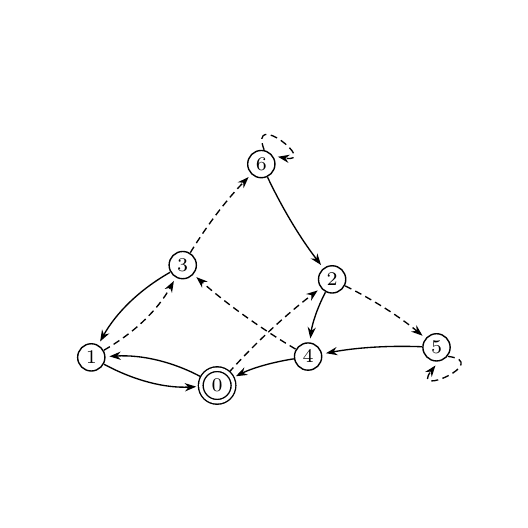
\begin{tikzpicture}[x=1cm,y=1cm,
  f1atlas state/.style={circle,draw=black,fill=white,line width=.5pt,inner sep=0pt,font=\fontsize{7}{8}\selectfont},
  f1atlas root/.style={f1atlas state,double,double distance=.42mm},
  f1atlas port0/.style={-{Stealth[length=1.45mm,width=1.05mm]},draw=black,line width=.48pt},
  f1atlas port1/.style={f1atlas port0,dash pattern=on 2.5pt off 1.6pt},
  f1atlas label/.style={font=\fontsize{6}{7}\selectfont,fill=white,inner sep=.4pt}
]
\path[use as bounding box] (-3,-3) rectangle (3,3);
% edge 0 0 1
\draw[f1atlas port0] (-0.78696,-1.44041) .. controls (-1.15753,-1.24056) and (-1.54917,-1.15196) .. (-1.96188,-1.17459);
% edge 0 1 2
\draw[f1atlas port1] (-0.44732,-1.38154) .. controls (-0.09993,-0.99568) and (0.27697,-0.64744) .. (0.68338,-0.33684);
% edge 1 0 0
\draw[f1atlas port0] (-2.02982,-1.27486) .. controls (-1.63893,-1.48566) and (-1.24866,-1.58038) .. (-0.85899,-1.55901);
% edge 1 1 3
\draw[f1atlas port1] (-2.03183,-1.09597) .. controls (-1.64235,-0.87448) and (-1.34607,-0.58146) .. (-1.14301,-0.21692);
% edge 2 0 4
\draw[f1atlas port0] (0.78148,-0.36046) .. controls (0.67775,-0.55969) and (0.61389,-0.75549) .. (0.58988,-0.94785);
% edge 2 1 5
\draw[f1atlas port1] (1.03207,-0.27883) .. controls (1.39728,-0.46022) and (1.72487,-0.67140) .. (2.01482,-0.91236);
% edge 3 0 1
\draw[f1atlas port0] (-1.19118,-0.10658) .. controls (-1.58066,-0.32807) and (-1.87694,-0.62109) .. (-2.08001,-0.98563);
% edge 3 1 6
\draw[f1atlas port1] (-0.93452,0.14226) .. controls (-0.71457,0.50261) and (-0.46777,0.82271) .. (-0.19412,1.10256);
% edge 4 0 0
\draw[f1atlas port0] (0.37896,-1.20570) .. controls (0.09676,-1.25036) and (-0.14826,-1.32408) .. (-0.35611,-1.42685);
% edge 4 1 3
\draw[f1atlas port1] (0.40267,-1.08241) .. controls (-0.05851,-0.80790) and (-0.47866,-0.50314) .. (-0.85778,-0.16813);
% edge 5 0 4
\draw[f1atlas port0] (2.00785,-1.05231) .. controls (1.58275,-1.03495) and (1.17620,-1.06239) .. (0.78818,-1.13461);
% edge 5 1 5
\draw[f1atlas port1] (2.33698,-1.17454) .. controls (2.89658,-1.23991) and (1.85694,-1.70479) .. (2.17858,-1.29021);
% edge 6 0 2
\draw[f1atlas port0] (0.04650,1.10082) .. controls (0.24105,0.69168) and (0.46742,0.32004) .. (0.72562,-0.01410);
% edge 6 1 6
\draw[f1atlas port1] (0.00284,1.44870) .. controls (-0.19556,1.97601) and (0.69414,1.26511) .. (0.17825,1.36094);
% state 0
\node[f1atlas root,minimum size=4.1538mm] (q0) at (-0.59400,-1.54447) {$ 0 $};
% state 1
\node[f1atlas state,minimum size=3.4615mm] (q1) at (-2.19231,-1.18723) {$ 1 $};
% state 2
\node[f1atlas state,minimum size=3.4615mm] (q2) at (0.86673,-0.19670) {$ 2 $};
% state 3
\node[f1atlas state,minimum size=3.4615mm] (q3) at (-1.03070,-0.01532) {$ 3 $};
% state 4
\node[f1atlas state,minimum size=3.4615mm] (q4) at (0.56131,-1.17684) {$ 4 $};
% state 5
\node[f1atlas state,minimum size=3.4615mm] (q5) at (2.19231,-1.05985) {$ 5 $};
% state 6
\node[f1atlas state,minimum size=3.4615mm] (q6) at (-0.03278,1.26755) {$ 6 $};
\end{tikzpicture}
}\par\smallskip
{\small (d) Rooted class 4; underlying shape 1.}\par
\end{minipage}\hfill
\par\vspace{3mm}
\clearpage
{\Large\bfseries Extremal Family 1 seed graphs}\par\vspace{2mm}
{\small $m=7$; $\max_G H(G)=34$. Complete collection: 8 rooted classes and 4 underlying shapes.}\par
\vspace{1.5mm}{\small Root $0$: double circle. Port $0$: solid; port $1$: dashed. Members of each underlying shape share one vertex embedding.}\par\vspace{3mm}
\noindent\hfill
\begin{minipage}[t]{.47\textwidth}\centering
\resizebox{8.2cm}{!}{% Family 1 rooted seed, m=7; key=0102010203040005030604060005.
% Requires \usepackage{tikz} and \usetikzlibrary{arrows.meta}.
% Score and global-maximality metadata belong in the surrounding caption.
\begin{tikzpicture}[x=1cm,y=1cm,
  f1atlas state/.style={circle,draw=black,fill=white,line width=.5pt,inner sep=0pt,font=\fontsize{7}{8}\selectfont},
  f1atlas root/.style={f1atlas state,double,double distance=.42mm},
  f1atlas port0/.style={-{Stealth[length=1.45mm,width=1.05mm]},draw=black,line width=.48pt},
  f1atlas port1/.style={f1atlas port0,dash pattern=on 2.5pt off 1.6pt},
  f1atlas label/.style={font=\fontsize{6}{7}\selectfont,fill=white,inner sep=.4pt}
]
\path[use as bounding box] (-3,-3) rectangle (3,3);
% edge 0 0 1
\draw[f1atlas port0] (-0.32190,0.57857) .. controls (-0.17302,0.82020) and (-0.06244,1.07426) .. (0.00987,1.34074);
% edge 0 1 2
\draw[f1atlas port1] (-0.22222,0.43639) .. controls (-0.01648,0.47900) and (0.18657,0.48589) .. (0.38692,0.45706);
% edge 1 0 1
\draw[f1atlas port0] (-0.09707,1.64138) .. controls (-0.65654,1.57489) and (0.24657,2.26869) .. (0.03010,1.79070);
% edge 1 1 2
\draw[f1atlas port1] (0.17322,1.41020) .. controls (0.34180,1.15917) and (0.46636,0.90396) .. (0.54691,0.64457);
% edge 2 0 3
\draw[f1atlas port0] (0.51236,0.27095) .. controls (0.38793,0.08579) and (0.30338,-0.10033) .. (0.25874,-0.28740);
% edge 2 1 4
\draw[f1atlas port1] (0.64364,0.24175) .. controls (0.70112,-0.12887) and (0.71374,-0.48556) .. (0.68148,-0.82833);
% edge 3 0 0
\draw[f1atlas port0] (0.12442,-0.34585) .. controls (0.01440,-0.11963) and (-0.11032,0.06357) .. (-0.24975,0.20375);
% edge 3 1 5
\draw[f1atlas port1] (0.20738,-0.69647) .. controls (0.21130,-1.02392) and (0.17482,-1.33092) .. (0.09796,-1.61749);
% edge 4 0 3
\draw[f1atlas port0] (0.58121,-0.89106) .. controls (0.52938,-0.78097) and (0.46652,-0.69942) .. (0.39266,-0.64641);
% edge 4 1 6
\draw[f1atlas port1] (0.47682,-1.08213) .. controls (0.15843,-1.12397) and (-0.14438,-1.12357) .. (-0.43159,-1.08095);
% edge 5 0 4
\draw[f1atlas port0] (0.17738,-1.71912) .. controls (0.33998,-1.57748) and (0.46469,-1.42505) .. (0.55150,-1.26183);
% edge 5 1 6
\draw[f1atlas port1] (-0.01811,-1.66456) .. controls (-0.09776,-1.41571) and (-0.24200,-1.24246) .. (-0.45082,-1.14482);
% edge 6 0 0
\draw[f1atlas port0] (-0.60887,-0.86964) .. controls (-0.50773,-0.51769) and (-0.45284,-0.18560) .. (-0.44422,0.12663);
% edge 6 1 5
\draw[f1atlas port1] (-0.60358,-1.22290) .. controls (-0.52392,-1.47175) and (-0.37969,-1.64499) .. (-0.17087,-1.74263);
% state 0
\node[f1atlas root,minimum size=4.1538mm] (q0) at (-0.43689,0.39192) {$ 0 $};
% state 1
\node[f1atlas state,minimum size=3.4615mm] (q1) at (0.07030,1.56346) {$ 1 $};
% state 2
\node[f1atlas state,minimum size=3.4615mm] (q2) at (0.61534,0.42418) {$ 2 $};
% state 3
\node[f1atlas state,minimum size=3.4615mm] (q3) at (0.20517,-0.51187) {$ 3 $};
% state 4
\node[f1atlas state,minimum size=3.4615mm] (q4) at (0.65986,-1.05808) {$ 4 $};
% state 5
\node[f1atlas state,minimum size=3.4615mm] (q5) at (0.03817,-1.84038) {$ 5 $};
% state 6
\node[f1atlas state,minimum size=3.4615mm] (q6) at (-0.65986,-1.04707) {$ 6 $};
\end{tikzpicture}
}\par\smallskip
{\small (e) Rooted class 5; underlying shape 3.}\par
\end{minipage}\hfill
\begin{minipage}[t]{.47\textwidth}\centering
\resizebox{8.2cm}{!}{% Family 1 rooted seed, m=7; key=0102010203040005050600060304.
% Requires \usepackage{tikz} and \usetikzlibrary{arrows.meta}.
% Score and global-maximality metadata belong in the surrounding caption.
\begin{tikzpicture}[x=1cm,y=1cm,
  f1atlas state/.style={circle,draw=black,fill=white,line width=.5pt,inner sep=0pt,font=\fontsize{7}{8}\selectfont},
  f1atlas root/.style={f1atlas state,double,double distance=.42mm},
  f1atlas port0/.style={-{Stealth[length=1.45mm,width=1.05mm]},draw=black,line width=.48pt},
  f1atlas port1/.style={f1atlas port0,dash pattern=on 2.5pt off 1.6pt},
  f1atlas label/.style={font=\fontsize{6}{7}\selectfont,fill=white,inner sep=.4pt}
]
\path[use as bounding box] (-3,-3) rectangle (3,3);
% edge 0 0 1
\draw[f1atlas port0] (-0.53422,0.63194) .. controls (-0.38142,0.85527) and (-0.26572,1.09237) .. (-0.18711,1.34325);
% edge 0 1 2
\draw[f1atlas port1] (-0.43886,0.45692) .. controls (-0.26989,0.46149) and (-0.11008,0.43490) .. (0.04057,0.37715);
% edge 1 0 1
\draw[f1atlas port0] (-0.29363,1.62073) .. controls (-0.84107,1.48756) and (-0.02778,2.28475) .. (-0.18530,1.78423);
% edge 1 1 2
\draw[f1atlas port1] (-0.04193,1.39530) .. controls (0.09103,1.10185) and (0.17901,0.81101) .. (0.22201,0.52280);
% edge 2 0 3
\draw[f1atlas port0] (0.10042,0.19525) .. controls (-0.19812,0.00476) and (-0.45692,-0.20942) .. (-0.67597,-0.44730);
% edge 2 1 4
\draw[f1atlas port1] (0.34862,0.13482) .. controls (0.53565,-0.18793) and (0.67588,-0.51394) .. (0.76930,-0.84321);
% edge 3 0 0
\draw[f1atlas port0] (-0.77234,-0.44244) .. controls (-0.69348,-0.21274) and (-0.65473,-0.00338) .. (-0.65610,0.18563);
% edge 3 1 5
\draw[f1atlas port1] (-0.65011,-0.64693) .. controls (-0.52054,-0.66818) and (-0.41578,-0.70928) .. (-0.33583,-0.77022);
% edge 4 0 5
\draw[f1atlas port0] (0.65821,-1.00375) .. controls (0.45565,-0.93224) and (0.26238,-0.89895) .. (0.07840,-0.90390);
% edge 4 1 6
\draw[f1atlas port1] (0.65667,-1.12214) .. controls (0.34980,-1.22160) and (0.11979,-1.39553) .. (-0.03336,-1.64395);
% edge 5 0 0
\draw[f1atlas port0] (-0.19425,-0.73032) .. controls (-0.27716,-0.37504) and (-0.39073,-0.05964) .. (-0.53494,0.21588);
% edge 5 1 6
\draw[f1atlas port1] (-0.11678,-1.09128) .. controls (-0.07964,-1.28073) and (-0.07705,-1.45502) .. (-0.10901,-1.61414);
% edge 6 0 3
\draw[f1atlas port0] (-0.22204,-1.66858) .. controls (-0.34910,-1.34551) and (-0.50676,-1.05683) .. (-0.69499,-0.80253);
% edge 6 1 4
\draw[f1atlas port1] (0.02116,-1.78346) .. controls (0.32804,-1.68400) and (0.55805,-1.51006) .. (0.71119,-1.26165);
% state 0
\node[f1atlas root,minimum size=4.1538mm] (q0) at (-0.65801,0.45101) {$ 0 $};
% state 1
\node[f1atlas state,minimum size=3.4615mm] (q1) at (-0.11812,1.56346) {$ 1 $};
% state 2
\node[f1atlas state,minimum size=3.4615mm] (q2) at (0.25606,0.29456) {$ 2 $};
% state 3
\node[f1atlas state,minimum size=3.4615mm] (q3) at (-0.83229,-0.61705) {$ 3 $};
% state 4
\node[f1atlas state,minimum size=3.4615mm] (q4) at (0.83229,-1.06521) {$ 4 $};
% state 5
\node[f1atlas state,minimum size=3.4615mm] (q5) at (-0.15229,-0.91011) {$ 5 $};
% state 6
\node[f1atlas state,minimum size=3.4615mm] (q6) at (-0.15446,-1.84038) {$ 6 $};
\end{tikzpicture}
}\par\smallskip
{\small (f) Rooted class 6; underlying shape 4.}\par
\end{minipage}\hfill
\par\vspace{3mm}
\noindent\hfill
\begin{minipage}[t]{.47\textwidth}\centering
\resizebox{8.2cm}{!}{% Family 1 rooted seed, m=7; key=0102020304050006000604050103.
% Requires \usepackage{tikz} and \usetikzlibrary{arrows.meta}.
% Score and global-maximality metadata belong in the surrounding caption.
\begin{tikzpicture}[x=1cm,y=1cm,
  f1atlas state/.style={circle,draw=black,fill=white,line width=.5pt,inner sep=0pt,font=\fontsize{7}{8}\selectfont},
  f1atlas root/.style={f1atlas state,double,double distance=.42mm},
  f1atlas port0/.style={-{Stealth[length=1.45mm,width=1.05mm]},draw=black,line width=.48pt},
  f1atlas port1/.style={f1atlas port0,dash pattern=on 2.5pt off 1.6pt},
  f1atlas label/.style={font=\fontsize{6}{7}\selectfont,fill=white,inner sep=.4pt}
]
\path[use as bounding box] (-3,-3) rectangle (3,3);
% edge 0 0 1
\draw[f1atlas port0] (-0.65793,-0.74995) .. controls (-0.57186,-0.81555) and (-0.47922,-0.85649) .. (-0.38002,-0.87276);
% edge 0 1 2
\draw[f1atlas port1] (-0.83388,-0.39783) .. controls (-0.83546,-0.17805) and (-0.80182,0.03214) .. (-0.73295,0.23274);
% edge 1 0 2
\draw[f1atlas port0] (-0.19425,-0.73032) .. controls (-0.27716,-0.37504) and (-0.39608,-0.04942) .. (-0.55099,0.24655);
% edge 1 1 3
\draw[f1atlas port1] (-0.11678,-1.09128) .. controls (-0.07964,-1.28073) and (-0.07705,-1.45502) .. (-0.10901,-1.61414);
% edge 2 0 4
\draw[f1atlas port0] (-0.48562,0.38493) .. controls (-0.30624,0.31618) and (-0.13591,0.28398) .. (0.02537,0.28833);
% edge 2 1 5
\draw[f1atlas port1] (-0.60281,0.62718) .. controls (-0.51501,0.90742) and (-0.39688,1.15603) .. (-0.24843,1.37300);
% edge 3 0 0
\draw[f1atlas port0] (-0.22204,-1.66858) .. controls (-0.34910,-1.34551) and (-0.49989,-1.06611) .. (-0.67440,-0.83036);
% edge 3 1 6
\draw[f1atlas port1] (0.02116,-1.78346) .. controls (0.32804,-1.68400) and (0.55805,-1.51006) .. (0.71119,-1.26165);
% edge 4 0 0
\draw[f1atlas port0] (0.10042,0.19525) .. controls (-0.19812,0.00476) and (-0.44910,-0.20093) .. (-0.65252,-0.42183);
% edge 4 1 6
\draw[f1atlas port1] (0.34862,0.13482) .. controls (0.53565,-0.18793) and (0.67588,-0.51394) .. (0.76930,-0.84321);
% edge 5 0 4
\draw[f1atlas port0] (-0.09088,1.38087) .. controls (-0.04334,1.06222) and (0.04056,0.77019) .. (0.16082,0.50476);
% edge 5 1 5
\draw[f1atlas port1] (-0.09152,1.74615) .. controls (-0.31579,2.26299) and (0.60803,1.59703) .. (0.08802,1.66719);
% edge 6 0 1
\draw[f1atlas port0] (0.65821,-1.00375) .. controls (0.45565,-0.93224) and (0.26238,-0.89895) .. (0.07840,-0.90390);
% edge 6 1 3
\draw[f1atlas port1] (0.65667,-1.12214) .. controls (0.34980,-1.22160) and (0.11979,-1.39553) .. (-0.03336,-1.64395);
% state 0
\node[f1atlas root,minimum size=4.1538mm] (q0) at (-0.83229,-0.61705) {$ 0 $};
% state 1
\node[f1atlas state,minimum size=3.4615mm] (q1) at (-0.15229,-0.91011) {$ 1 $};
% state 2
\node[f1atlas state,minimum size=3.4615mm] (q2) at (-0.65801,0.45101) {$ 2 $};
% state 3
\node[f1atlas state,minimum size=3.4615mm] (q3) at (-0.15446,-1.84038) {$ 3 $};
% state 4
\node[f1atlas state,minimum size=3.4615mm] (q4) at (0.25606,0.29456) {$ 4 $};
% state 5
\node[f1atlas state,minimum size=3.4615mm] (q5) at (-0.11812,1.56346) {$ 5 $};
% state 6
\node[f1atlas state,minimum size=3.4615mm] (q6) at (0.83229,-1.06521) {$ 6 $};
\end{tikzpicture}
}\par\smallskip
{\small (g) Rooted class 7; underlying shape 4.}\par
\end{minipage}\hfill
\begin{minipage}[t]{.47\textwidth}\centering
\resizebox{8.2cm}{!}{% Family 1 rooted seed, m=7; key=0102030405060001000203040506.
% Requires \usepackage{tikz} and \usetikzlibrary{arrows.meta}.
% Score and global-maximality metadata belong in the surrounding caption.
\begin{tikzpicture}[x=1cm,y=1cm,
  f1atlas state/.style={circle,draw=black,fill=white,line width=.5pt,inner sep=0pt,font=\fontsize{7}{8}\selectfont},
  f1atlas root/.style={f1atlas state,double,double distance=.42mm},
  f1atlas port0/.style={-{Stealth[length=1.45mm,width=1.05mm]},draw=black,line width=.48pt},
  f1atlas port1/.style={f1atlas port0,dash pattern=on 2.5pt off 1.6pt},
  f1atlas label/.style={font=\fontsize{6}{7}\selectfont,fill=white,inner sep=.4pt}
]
\path[use as bounding box] (-3,-3) rectangle (3,3);
% edge 0 0 1
\draw[f1atlas port0] (-0.19547,-1.12504) .. controls (-0.22894,-1.29170) and (-0.23007,-1.45466) .. (-0.19885,-1.61393);
% edge 0 1 2
\draw[f1atlas port1] (-0.25395,-0.71587) .. controls (-0.41244,-0.41309) and (-0.52964,-0.09904) .. (-0.60556,0.22628);
% edge 1 0 3
\draw[f1atlas port0] (0.02116,-1.78346) .. controls (0.32804,-1.68400) and (0.55805,-1.51006) .. (0.71119,-1.26165);
% edge 1 1 4
\draw[f1atlas port1] (-0.26430,-1.69200) .. controls (-0.47085,-1.41297) and (-0.63202,-1.12624) .. (-0.74783,-0.83181);
% edge 2 0 5
\draw[f1atlas port0] (-0.48562,0.38493) .. controls (-0.30624,0.31618) and (-0.13591,0.28398) .. (0.02537,0.28833);
% edge 2 1 6
\draw[f1atlas port1] (-0.60281,0.62718) .. controls (-0.51501,0.90742) and (-0.39688,1.15603) .. (-0.24843,1.37300);
% edge 3 0 0
\draw[f1atlas port0] (0.65821,-1.00375) .. controls (0.45565,-0.93224) and (0.27391,-0.89864) .. (0.11300,-0.90297);
% edge 3 1 1
\draw[f1atlas port1] (0.65667,-1.12214) .. controls (0.34980,-1.22160) and (0.11979,-1.39553) .. (-0.03336,-1.64395);
% edge 4 0 0
\draw[f1atlas port0] (-0.68546,-0.72896) .. controls (-0.58104,-0.80855) and (-0.49061,-0.85462) .. (-0.41418,-0.86715);
% edge 4 1 2
\draw[f1atlas port1] (-0.83363,-0.43244) .. controls (-0.83538,-0.18958) and (-0.80182,0.03214) .. (-0.73295,0.23274);
% edge 5 0 3
\draw[f1atlas port0] (0.30645,0.11695) .. controls (0.40827,-0.24191) and (0.54499,-0.56941) .. (0.71659,-0.86555);
% edge 5 1 4
\draw[f1atlas port1] (0.13100,0.15875) .. controls (-0.10890,-0.10176) and (-0.36515,-0.31898) .. (-0.63775,-0.49292);
% edge 6 0 5
\draw[f1atlas port0] (-0.09088,1.38087) .. controls (-0.04334,1.06222) and (0.04056,0.77019) .. (0.16082,0.50476);
% edge 6 1 6
\draw[f1atlas port1] (-0.09152,1.74615) .. controls (-0.31579,2.26299) and (0.60803,1.59703) .. (0.08802,1.66719);
% state 0
\node[f1atlas root,minimum size=4.1538mm] (q0) at (-0.15229,-0.91011) {$ 0 $};
% state 1
\node[f1atlas state,minimum size=3.4615mm] (q1) at (-0.15446,-1.84038) {$ 1 $};
% state 2
\node[f1atlas state,minimum size=3.4615mm] (q2) at (-0.65801,0.45101) {$ 2 $};
% state 3
\node[f1atlas state,minimum size=3.4615mm] (q3) at (0.83229,-1.06521) {$ 3 $};
% state 4
\node[f1atlas state,minimum size=3.4615mm] (q4) at (-0.83229,-0.61705) {$ 4 $};
% state 5
\node[f1atlas state,minimum size=3.4615mm] (q5) at (0.25606,0.29456) {$ 5 $};
% state 6
\node[f1atlas state,minimum size=3.4615mm] (q6) at (-0.11812,1.56346) {$ 6 $};
\end{tikzpicture}
}\par\smallskip
{\small (h) Rooted class 8; underlying shape 4.}\par
\end{minipage}\hfill
\par\vspace{3mm}
\end{document}
